\chapter{Rapport}

    \section{Internettets historie}
        Internettet blev opfundet den 29 oktober 1969, af et hold forskere på UCLA (University of California). Det blev dengang kaldet ARPANET, hvilket senere blev til det, der i dag er kendt som internettet. 
        Den første besked sendt fra internettet var bogstavet I, og dengang bestod hele internettet af en netværksnode mellem UCLA og SRI (Science and Research Initiative). 
        Den tredje besked var et g, hvilket fik hele systemet til at bryde sammen. 
        Da man genoplivede systemet var forbindelsen dog stabil, og efterfølgende inden året var omme opstod der et fungerende netværk bestående af 4 computere.
        Allerede i 1971 blev den første computervirus opfundet. Virussen blev kaldt creeper og den kopierede sig selv over netværket, hvorefter den gav beskeden ”I’m the creeper, catch me if you can”. Senere samme år blev den første email introduceret af Ray Tomlinson.\\
        I oktober 1972 blev ARPANET for første gang demonstreret offentligt, under ICCC konferencen, (International Computer Communication Conference) af Bob Metcalfe. I september 1973 blev ARPANET erstattet med Transmission Control Protocol/Internet Protocol (TCP/IP), hvorefter internettet blev globalt, og DARPA (Denfense Advanced Research Projects Agency) åbnede 3 nye uafhængige TCP/IP institutioner i Standford University, London University og BBN.
        1980, Tim Berners-Lee udvikler et program der registrerede links imellem computerne og projekterne i CERN. 
        Programmet blev kaldt ENQUIRE, og det var her ideen om World Wide Web begyndte at forme sig, og allerede efter 3 år viser en undersøgelse af Louis Harris and Associates Inc at 10\% af amerikanske voksne ejer en computer og at ud af dem har 14\% adgang til et modem som kan sende og modtage information, altså ca. 1,4\% af voksne amerikanere havde adgang til internettet. 
        I marts 1985 åbnes den første kommercielle internet domæne af Symbolics.com, et computer firma i Massachusetts, og
        i september 1988 åbnes det første Interhop trade show, hvilket er den første hjemmeside, der sammensætter 50 forskellige online forretninger på TCP/IP.\\
        Et par måneder senere introducerer Robert Tappan Morris, hvad der senere bliver kaldet The Morris Worm, hvilket var en computer virus der ramte og beskadigede ca. 10\% af alle computere forbundet med internettet. Han var den første person som nogensinde blev dømt for online hærværk/svindel. Han startede senere et firma, som han solgte til Yahoo i 1998, han underviser i dag på MIT. I 1990 udvikles den første Internet Search Engine kaldet Archie af Alan Emtage, året efter udgiver Tim Berners-Lee koden for World Wide Web på internettet og den første hjemmeside på internettet kommer online fra SLAC National Accelerator Laboratory. November 1993, det første videokamera bliver tilsluttet til internettet i Cambridge University i London, hvilket er det første Webcam, og sommeren efter finder den første online transaktion sted, der bliver bestilt og betalt for en pizza fra Pizzahut.\\\\
        I 1995 fortæller en undersøgelse af The Pew Research Center at 14\% af alle voksne amerikanere er online, året efter udgiver Nokia, en mobiltelefon Nokia 9000 Communicator, den første telefon med en webbrowser. Senere sammen år introducerer Ethan Zuckerman den første pop-up reklame, hvilket kan senere undskyldte mange gange for, da dette blev kendt som ”The Internet’s Original Sin”. I år 1998 registrerer Google index’et 26 millioner webpages, 2 år senere bliver dette 1 milliard og 10 år senere 1 trillion. Marts 2007 Estonia bliver det første land, der bruger internettet til deres parlaments afstemning. December 2012, der bliver handlet for mere en 1 trillion dollars på internettet årligt, og mindre en to år senere er der mere en 3 milliarder mennesker verden over er på internettet.\autocite{gilpress2015}\\

    
    
    \section{Internet of Things}
        Begrebet Internet of Things (IoT) blev skabt i 1999 af MIT Auto-ID Center grundlæggere, Kevin Ashton og David L. Brock.\autocite{Hashmi2017} Auto-ID er en bred vifte af teknologier brugt i industrier til at øge effektiviteten, automation samt reduktion af fejl. Disse teknologier kan være sensore, stemme genkendelse, stregkode osv.
        Siden 2003 har Auto-ID teknologi ændret sig til hovedsageligt at være Radio Frequency Identification(RFID) fra sensore, stemme genkendeldse og stregkoder osv.\autocite{Sundmaeker2010}. Oprindeligt var MIT Auto-ID Center industri sponsoreret forsknings og udviklingscenter, hvor alt deres arbejde blev frit tilgængeligt. Centeres vision var:\\
        \textit{``The Auto-ID Center envisions a world in which all electronic devices are networked and every object, whether it is physical or electronic, is electronically tagged with information pertinent to that object.''} -\autocite[Kapitel 2,p. ~4]{Sarma2001} Visionen var altså at det var muligt at forbinde alle fysiske objekter til et netværk. 
        I oktober 2003 skiftede MIT Auto-ID Center navn til Cambridge Auto-ID Lab og blev lukket. Centeret blev delt i Auto-ID Labs forsknings enhed og EPCglobal kommercielt enhed eget af UCC og EAN.\autocite{Sundmaeker2010}\\
        Formålet med Auto-ID Labs i dag er at udvikle et netværk, som forbinder computer til objekter. Dette er ikke blot hardware eller software som er forbundet på et netværk, men alt hvad der benyttes til at skabe IoT. Det vil sige hardware, netværk software og protokoller, sprog til at beskrive objekter således at computer kan kommunikere. Det er ikke et nyt internet, men elementer bygget oven på eksisterende internet teknologi, som gøre det muligt at spore og dele information på tværs af\todo{Omformulering af overstående} internettet.\autocite{Sundmaeker2010} \\
        \begin{figure}[H]
            \centering
                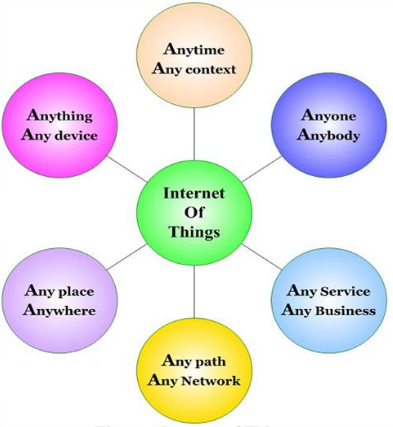
\includegraphics[0.55]{figures/IoT_definition.png}
            \caption{IoT kommunikation.\autocite{Sundmaeker2010}}\label{fig:IOTkom}
        \end{figure}
        Ved at overveje det nævnte kan IoT enheder defineres som enheder eller ting, som gennem trådløse forbindelser samt kabelforbindelser i et netværk er i stand til at samarbejde med andre forbundet enheder, se figur \ref{fig:IOTkom}. IoT enhederne er i stand til at skabe flydende kommunikation og kontekstuel service.\autocite{Hashmi2017}
        IoT enheder kan have følgende kommunikations mønstre: menneske til menneske, menneske til enhed, enhed til enhed.\\
        Dette vil altså sige at IoT enheder kan defineres som alt fra General Purpose Devices (Computere, printere, mobiltelefoner eller lign.) (GPD) til kaffemaskiner og toiletter tilkoblet wi-fi eller ethernet. Da GDP enheder er produceret af firmaer som Apple, hp, samsung og lenovo, er disse ofte produceret med kundernes sikkerhed i fokus. Rapporten har på baggrund af dette valgt at eksludere GPD enheder fra rapportens arbejdsområde, da disse ofte får software opdateringer der øger sikkerheden på produkterene.
        Arbejdsområdet indenfor IoT er altså reduceret til at være fokuseret på de produkter der kun nyligt er kommet på markedet, så som kaffemaskiner og toiletter med internet funktioner. \\

